\section{伊辛模型的 Bethe 与 Bragg--Williams 描述}

\subsection{模型、假设与记号}

考虑无向图 \(G=(V,E)\) 上的零场或有场伊辛模型。每个顶点 \(i\in V\) 携带一个二值自旋
\(\sigma_i=\pm1\)，微观态记为 \(\{\sigma_i\}\)，哈密顿量取为
\begin{equation*}
	\mathcal H[\{\sigma_i\}]
	= -J\sum_{(ij)\in E}\sigma_i\sigma_j-\mu B\sum_{i\in V}\sigma_i .
\end{equation*}
这里 \(J>0\) 表示铁磁耦合，\(\mu B\) 是单个自旋在外场中的能量尺度。本文的 \(q\) 始终表示配位数，即每个正则顶点与 \(q\) 个邻居相连；因此在 \(q\)-正则树上顶点度就是 \(q\)，边数在热力学极限中为 \(qN/2\)。在一般不规则树上，顶点 \(i\) 的度记为 \(d_i\)。

除特别说明外，以下约定统一为
\begin{equation*}
	m=\langle\sigma_i\rangle=p_+-p_-,\qquad
t=\frac{T-T_c}{T_c},\qquad
h=\frac{\mu B}{kT_c}.
\end{equation*}
其中 \(T_c\) 的数值取决于所讨论的近似：在 Bethe 小节中它指 Bethe 临界温度，在 Bragg--Williams 小节中它指相应的平均场临界温度。因而 \(t\) 的定义形式相同，但两个小节中的温度尺度不能混用。另记
\begin{equation*}
	\beta=\frac{1}{kT},\qquad \gamma=\beta J.
\end{equation*}

先在有限树上讨论严格等式，再取无限 \(q\)-正则树的平移不变热力学解。对于真正的有限维晶格，Bethe 结果应理解为局部树近似或无环基准，而不是一般意义下的精确解。

\subsection{树图概率分解为何严格}

\subsubsection{链式法则与唯一父节点}

任选有限树上的根节点 \(r\)，每个 \(i\neq r\) 都有唯一父节点 \(\pi(i)\)。对任意联合分布，链式法则给出
\begin{equation*}
	P(\{\sigma_i\})
	=P(\sigma_r)\prod_{i\neq r}P(\sigma_i\mid \sigma_{\pi(i)},\text{其余祖先状态}).
\end{equation*}
在树图的马尔可夫模型中，给定父节点后，子树内部与其余分支条件独立，因此上式严格化为
\begin{equation*}
	P(\{\sigma_i\})
	=P(\sigma_r)\prod_{i\neq r}P(\sigma_i\mid\sigma_{\pi(i)}).
\end{equation*}
将条件概率改写成边缘概率，得到
\begin{equation*}
	P(\{\sigma_i\})
	=P(\sigma_r)\prod_{i\neq r}
	\frac{P(\sigma_i,\sigma_{\pi(i)})}{P(\sigma_{\pi(i)})}
	=\frac{\displaystyle\prod_{(ij)\in E}P(\sigma_i,\sigma_j)}
	{\displaystyle\prod_{i\in V}P(\sigma_i)^{d_i-1}} .
\end{equation*}
最后一个式子中，顶点 \(i\) 作为父节点出现 \(d_i-1\) 次；根节点的额外因子正好使计数成立。这里的 \(P(\sigma_i)\) 和 \(P(\sigma_i,\sigma_j)\) 分别是单点和相邻点联合概率，满足
\begin{equation*}
	\sum_{\sigma_i}P(\sigma_i)=1,\qquad
	\sum_{\sigma_i,\sigma_j}P(\sigma_i,\sigma_j)=1,
\end{equation*}
\begin{equation*}
	P(\sigma_i,\sigma_j)=P(\sigma_j,\sigma_i),\qquad
	\sum_{\sigma_j}P(\sigma_i,\sigma_j)=P(\sigma_i).
\end{equation*}
这些边缘一致性条件是局域概率能够拼成全局树图概率的必要条件。直接逐层求和也可以验证
\begin{equation*}
	\sum_{\{\sigma_i\}}P(\{\sigma_i\})=1.
\end{equation*}

在有环图上，给定一条边或一个邻居后，两个分支仍可能通过另一条路径相关，因此上述分解一般不再是精确的。Bethe 近似所做的事情，是把一般图上的局域概率仍然代入同一个树图熵泛函；近似误差的主要来源正是被忽略的环图关联。

\subsubsection{Bethe 熵}

对树图概率取 Shannon 熵，利用前述严格分解，有
\begin{align*}
	\frac{S}{k}
	&=-\sum_{\{\sigma_i\}}P(\{\sigma_i\})\ln P(\{\sigma_i\})\\
	&=-\sum_{(ij)\in E}\sum_{\sigma_i,\sigma_j}
	P(\sigma_i,\sigma_j)\ln P(\sigma_i,\sigma_j)
	+\sum_{i\in V}(d_i-1)\sum_{\sigma_i}
	P(\sigma_i)\ln P(\sigma_i).
\end{align*}
在 \(q\)-正则树的平移不变状态中，记单点概率为 \(p_\sigma\)，边概率为 \(p_{\sigma\sigma'}\)，则每个格点对应 \(q/2\) 条边，因而
\begin{equation*}
	\frac{S}{Nk}
	=-\frac q2\sum_{\sigma,\sigma'}p_{\sigma\sigma'}\ln p_{\sigma\sigma'}
	+(q-1)\sum_\sigma p_\sigma\ln p_\sigma .
\end{equation*}

\subsection{Bethe 自由能与自洽方程}

\subsubsection{局域概率参数化}

对二态伊辛模型，令
\begin{equation*}
	p_+=P(\sigma=+1),\qquad p_-=P(\sigma=-1),
\end{equation*}
并令 \(p_{++},p_{--},p_{+-}=p_{-+}\) 表示一条无向边上相应自旋组合的概率。它们满足
\begin{equation*}
	p_++p_-=1,\qquad
	p_{++}+p_{--}+2p_{+-}=1,
\end{equation*}
\begin{equation*}
	p_+-p_-=m,\qquad
	p_{++}=\frac{1+m-2p_{+-}}2,\qquad
	p_{--}=\frac{1-m-2p_{+-}}2.
\end{equation*}
因此在平移不变假设下，自由变量可选为 \(m\) 和 \(p_{+-}\)。物理概率域还要求
\[
	|m|\leq1,\qquad
	0\leq p_{+-}\leq\frac{1-|m|}{2}.
\]

平均能量密度为
\begin{equation*}
	\frac EN
	=-\frac{qJ}{2}
	\left(p_{++}+p_{--}-p_{+-}-p_{-+}\right)
	-\mu B(p_+-p_-)
	=-\frac{qJ}{2}\left(1-4p_{+-}\right)-\mu Bm .
\end{equation*}
与 Bethe 熵合在一起，得到无量纲自由能
\begin{align*}
	\Phi=\frac{F}{NkT_c}
	&=(1+t)\Bigg[
	\frac q2\left(
	p_{++}\ln p_{++}+p_{--}\ln p_{--}+2p_{+-}\ln p_{+-}\right)\\
	&\qquad\qquad
	-(q-1)\left(
	p_+\ln p_++p_-\ln p_-\right)\Bigg]\\
	&\quad-\frac{qJ}{2kT_c}(1-4p_{+-})-hm .
\end{align*}
对本小节的 Bethe 临界温度，后面将证明
\begin{equation*}
	T_c=T_c^{\mathrm B}
	=\frac{2J}{k}\left(\ln\frac{q}{q-2}\right)^{-1},
\qquad
\gamma=\frac{J}{kT}
	=\frac{1}{2(1+t)}\ln\frac{q}{q-2}.
\end{equation*}
将 \(p_{++},p_{--}\) 写成 \(m,p_{+-}\) 后，\(\Phi\) 就是 \(\Phi(m,t,p_{+-},h)\)。在内部极值点满足
\begin{equation*}
	\frac{\partial\Phi}{\partial p_{+-}}=0,\qquad
	\frac{\partial\Phi}{\partial m}=0.
\end{equation*}
解得
\begin{equation*}
	p_{+-}
	=\frac{1-m^2}
	{2\left[1+\sqrt{m^2+(1-m^2)
	\left(\dfrac q{q-2}\right)^{\frac{2}{1+t}}}\right]},
\end{equation*}
\begin{equation*}
	h=\frac{1+t}{2}\left[
	\frac q2\ln\frac{1+m-2p_{+-}}{1-m-2p_{+-}}
	-(q-1)\ln\frac{1+m}{1-m}\right].
\end{equation*}
第一条方程确定给定磁化强度下最优的边关联，第二条方程则是外场与磁化强度的状态方程。

\subsubsection{腔场变量与自洽方程}

为了把方程化为更适合分析的形式，引入腔场参数 \(a\)，令
\begin{equation*}
	m=\frac{\sinh(2a)}{\cosh(2a)+e^{-2\gamma}}.
\end{equation*}
则
\begin{align*}
	p_{+-}&=\frac{e^{-2\gamma}}
	{2\left(\cosh(2a)+e^{-2\gamma}\right)},\\
	p_{++}&=\frac{e^{2a}}
	{2\left(\cosh(2a)+e^{-2\gamma}\right)},\qquad
	p_{--}=\frac{e^{-2a}}
	{2\left(\cosh(2a)+e^{-2\gamma}\right)},\\
	p_\pm&=\frac{e^{-2\gamma}+e^{\pm2a}}
	{2\left(\cosh(2a)+e^{-2\gamma}\right)}.
\end{align*}
外场状态方程成为
\begin{equation*}
	h=(1+t)\left[
	a-\frac{q-1}{2}
	\ln\frac{\cosh(a+\gamma)}{\cosh(a-\gamma)}
	\right].
\end{equation*}
这里 \(a\) 不是外场本身，而是包含外场和来自 \(q-1\) 个分支的腔场变量。定义
\[
	\widetilde h=\frac{h}{1+t}=\beta\mu B,
\]
则上式也可写成
\[
	\widetilde h
	=a-\frac{q-1}{2}
	\ln\frac{\cosh(a+\gamma)}{\cosh(a-\gamma)}.
\]

从中心节点的角度看，去掉中心后其 \(q\) 个分支互不相连；给定中心自旋时，各分支条件独立。这是 Bethe--Peierls 腔场构造成立的结构原因。把中心自旋 \(\sigma_0\) 及其 \(q\) 个邻居组成一个集团，令集团外的影响由 \(B'\) 表示，则
\begin{equation*}
	\mathcal H_q
	=-J\sigma_0\sum_{i=1}^q\sigma_i
	-\mu B\sigma_0
	-\mu(B+B')\sum_{i=1}^q\sigma_i .
\end{equation*}
记
\begin{equation*}
	\widetilde h=\beta\mu B,\qquad
	\widetilde h'=\beta\mu B',\qquad
	\gamma=\beta J .
\end{equation*}
局域配分函数为
\begin{align*}
	Q&=\sum_{\sigma_0,\{\sigma_i\}}
	\exp\left[
	\widetilde h\sigma_0+
	\left(\widetilde h+\widetilde h'
	+\gamma\sigma_0\right)\sum_{i=1}^q\sigma_i
	\right]\\
	&=Q_++Q_-,
\end{align*}
其中
\begin{equation*}
	Q_\pm=e^{\pm\widetilde h}
	\left[2\cosh\left(\widetilde h+\widetilde h'\pm\gamma\right)\right]^q.
\end{equation*}
因此
\begin{equation*}
	\langle\sigma_0\rangle
	=\frac{Q_+-Q_-}{Q_++Q_-},
\end{equation*}
\begin{equation*}
	\langle\sigma_i\rangle
	=\frac1q\frac{\partial\ln Q}{\partial\widetilde h'}
	=\frac{
	Q_+\tanh(\widetilde h+\widetilde h'+\gamma)
	+Q_-\tanh(\widetilde h+\widetilde h'-\gamma)}
	{Q_++Q_-}.
\end{equation*}
平移不变性要求 \(\langle\sigma_0\rangle=\langle\sigma_i\rangle\)，从而
\begin{equation*}
	e^{2\widetilde h'}
	=\left[
	\frac{\cosh(\widetilde h+\widetilde h'+\gamma)}
	{\cosh(\widetilde h+\widetilde h'-\gamma)}
	\right]^{q-1}.
\end{equation*}
令 \(a=\widetilde h+\widetilde h'\)，就重新得到前述状态方程。

\subsection{临界性、响应函数与临界展开}

\subsubsection{磁化率与临界条件}

由 \(m(a,\gamma)\) 和 \(h(a,\gamma)\) 对 \(a\) 求导，可以得到固定 \(t\) 下的磁化率
\begin{equation*}
	\chi=\left(\frac{\partial m}{\partial h}\right)_t
	=\frac{
	4\left[1+e^{-2\gamma}\cosh(2a)\right]
	\left[\cosh(2a)+e^{-2\gamma}\right]^{-2}}
	{(1+t)\left[
	2-(q-1)\left(\tanh(a+\gamma)-\tanh(a-\gamma)\right)
	\right]} .
\end{equation*}
在对称态 \(a=0\) 附近，磁化率的发散由状态方程的线性系数为零决定。等价地，
\begin{equation*}
	(q-1)\tanh\gamma=1.
\end{equation*}
因为
\begin{equation*}
	\tanh\left[\frac12\ln\frac q{q-2}\right]=\frac1{q-1},
\end{equation*}
这正对应 \(t=0\)，即
\[
	T_c^{\mathrm B}
	=\frac{2J}{k}\left(\ln\frac q{q-2}\right)^{-1}.
\]
这里的临界温度是无限 \(q\)-正则树上平移不变解的临界温度；它不应直接等同于相同配位数的有限维晶格临界温度。

\subsubsection{临界点附近的状态方程}

在临界温度附近 \(m\) 很小，由参数关系展开得
\begin{equation*}
	a=\frac{1+e^{-2\gamma}}2m+\mathcal O(m^3),
\end{equation*}
\begin{equation*}
	h=\frac{(1+t)(1+e^{-2\gamma})}{2}
	\left[1-(q-1)\tanh\gamma\right]m
	+\mathcal O(m^3).
\end{equation*}
因而在临界等温线上
\begin{equation*}
	\left.m\right|_{t=0}
	=\left(\frac{3q^2}{(q-1)(q-2)}\right)^{1/3}h^{1/3}.
\end{equation*}
在零外场下，非零磁化强度由
\begin{equation*}
	\left[
	a-\frac{q-1}{2}
	\ln\frac{\cosh(a+\gamma)}{\cosh(a-\gamma)}
	\right]_{h=0}=0
\end{equation*}
确定。临界点附近的结果为
\begin{align*}
\left.m\right|_{h=0}
&=
\begin{cases}
	0,&t\gtrsim0,\\
\displaystyle
\pm\sqrt{\frac32\frac{q^2}{q-1}
\ln\frac q{q-2}}\,(-t)^{1/2},&t\lesssim0,
\end{cases}\\
\left.\chi\right|_{h=0}
&=
\begin{cases}
\displaystyle
\left[\frac12(q-2)\ln\frac q{q-2}\right]^{-1}t^{-1},
	&t\gtrsim0,\\
\displaystyle
\left[(q-2)\ln\frac q{q-2}\right]^{-1}(-t)^{-1},
	&t\lesssim0.
\end{cases}
\end{align*}
这给出 Bethe 解的平均场型临界指数
\[
\beta_{\mathrm{crit}}=\frac12,\qquad
\gamma_{\mathrm{crit}}=1,\qquad
\delta=3.
\]
这里的 \(\beta_{\mathrm{crit}}\) 是临界指数，不应与热力学中的 \(\beta=1/(kT)\) 混淆。

\subsubsection{能量、热容与两侧振幅}

在 \(h=0\) 时，能量和热容可以写成
\begin{align*}
\left.\frac{E}{NkT_c}\right|_{h=0}
&=-\frac q4
\frac{\cosh(2a)-e^{-2\gamma}}
{\cosh(2a)+e^{-2\gamma}}
\ln\frac q{q-2},\\
\left.\frac{C}{Nk}\right|_{h=0}
&=\left.\frac1{Nk}\frac{\d E}{\d T}\right|_{h=0}\\
&=\left(\frac{T_c}{T}\right)^2
\frac{qe^{-2\gamma}}
{2\left[\cosh(2a)+e^{-2\gamma}\right]^2}
\left(\ln\frac q{q-2}\right)^2\\
&\quad\times\left[
\cosh(2a)+
\frac{(q-1)\sinh^2(2a)}
{\cosh(2a)+\cosh(2\gamma)-(q-1)\sinh(2\gamma)}
\right].
\end{align*}
临界点两侧的展开为
\begin{align*}
\left.\frac{E}{NkT_c}\right|_{h=0}
&=
\begin{cases}
\displaystyle-\frac14\frac q{q-1}\ln\frac q{q-2}
+t\frac{q^2(q-2)}{8(q-1)^2}
\left(\ln\frac q{q-2}\right)^2,&t\gtrsim0,\\[6pt]
\displaystyle-\frac14\frac q{q-1}\ln\frac q{q-2}
+t\frac{q^2(q-2)(3q-2)}{8(q-1)^2}
\left(\ln\frac q{q-2}\right)^2,&t\lesssim0,
\end{cases}\\
\left.\frac{C}{Nk}\right|_{h=0}
&=
\begin{cases}
\displaystyle
\frac{q^2(q-2)}{8(q-1)^2}
\left(\ln\frac q{q-2}\right)^2,&t\gtrsim0,\\[6pt]
\displaystyle
\frac{q^2(q-2)(3q-2)}{8(q-1)^2}
\left(\ln\frac q{q-2}\right)^2,&t\lesssim0.
\end{cases}
\end{align*}
树图 Bethe 解在这里表现为热容的有限跃变，振幅和热容跃变的数值依赖于 \(q\)。

\subsubsection{自由能的 Landau 展开}

把 Bethe 自由能在 \(t\to0,m\to0\) 处展开，得到
\begin{align*}
\Phi
&=-mh+
\left(-\ln2+\frac q4\ln\frac{q(q-2)}{(q-1)^2}\right)\\
&\quad+\left[
-\ln2+\frac{q}{4(q-1)}
\left((q-2)\ln(q-2)-2(q-1)\ln(q-1)+q\ln q\right)
\right]t\\
&\quad-\frac{q^2(q-2)}{16(q-1)^2}
\left(\ln\frac q{q-2}\right)^2t^2
+\frac{q-2}{4}\ln\frac q{q-2}\,tm^2\\
&\quad+\frac{(q-2)(q-1)}{12q^2}m^4
+\mathcal O(t^3,t^2m^2,tm^4).
\end{align*}
写成
\begin{equation*}
\Phi=-hm+(a_0+a_1t+a_2t^2)+b_1tm^2+c_0m^4
+\mathcal O(t^3,t^2m^2,tm^4),
\end{equation*}
其中
\begin{equation*}
	a_2=-\frac{q^2(q-2)}{16(q-1)^2}
	\left(\ln\frac q{q-2}\right)^2,\quad
	b_1=\frac{q-2}{4}\ln\frac q{q-2},\quad
	c_0=\frac{(q-2)(q-1)}{12q^2}.
\end{equation*}
极值条件为
\begin{equation*}
	\frac{\partial\Phi}{\partial m}=0
	\quad\Longrightarrow\quad
	h=2b_1tm+4c_0m^3.
\end{equation*}
因此
\begin{align*}
\left.m\right|_{t=0}
&=\left(\frac1{4c_0}\right)^{1/3}h^{1/3},\\
\left.m\right|_{h=0}
&=
\begin{cases}
	0,&t\gtrsim0,\\
\displaystyle\sqrt{\frac{b_1}{2c_0}}\,(-t)^{1/2},&t\lesssim0,
\end{cases}\\
\left.\chi\right|_{h=0}
&=
\begin{cases}
\displaystyle\frac1{2b_1}t^{-1},&t\gtrsim0,\\
\displaystyle\frac1{4b_1}(-t)^{-1},&t\lesssim0,
\end{cases}\\
\left.\frac C{Nk}\right|_{h=0}
&=-\frac{\d^2\Phi(t,m(t))}{\d t^2}\\
&=
\begin{cases}
-2a_2,&t\gtrsim0,\\
\displaystyle-2a_2+\frac{b_1^2}{2c_0},&t\lesssim0.
\end{cases}
\end{align*}
\begin{figure}[htbp]
	\centering
	\begin{subfigure}[b]{0.49\textwidth}
		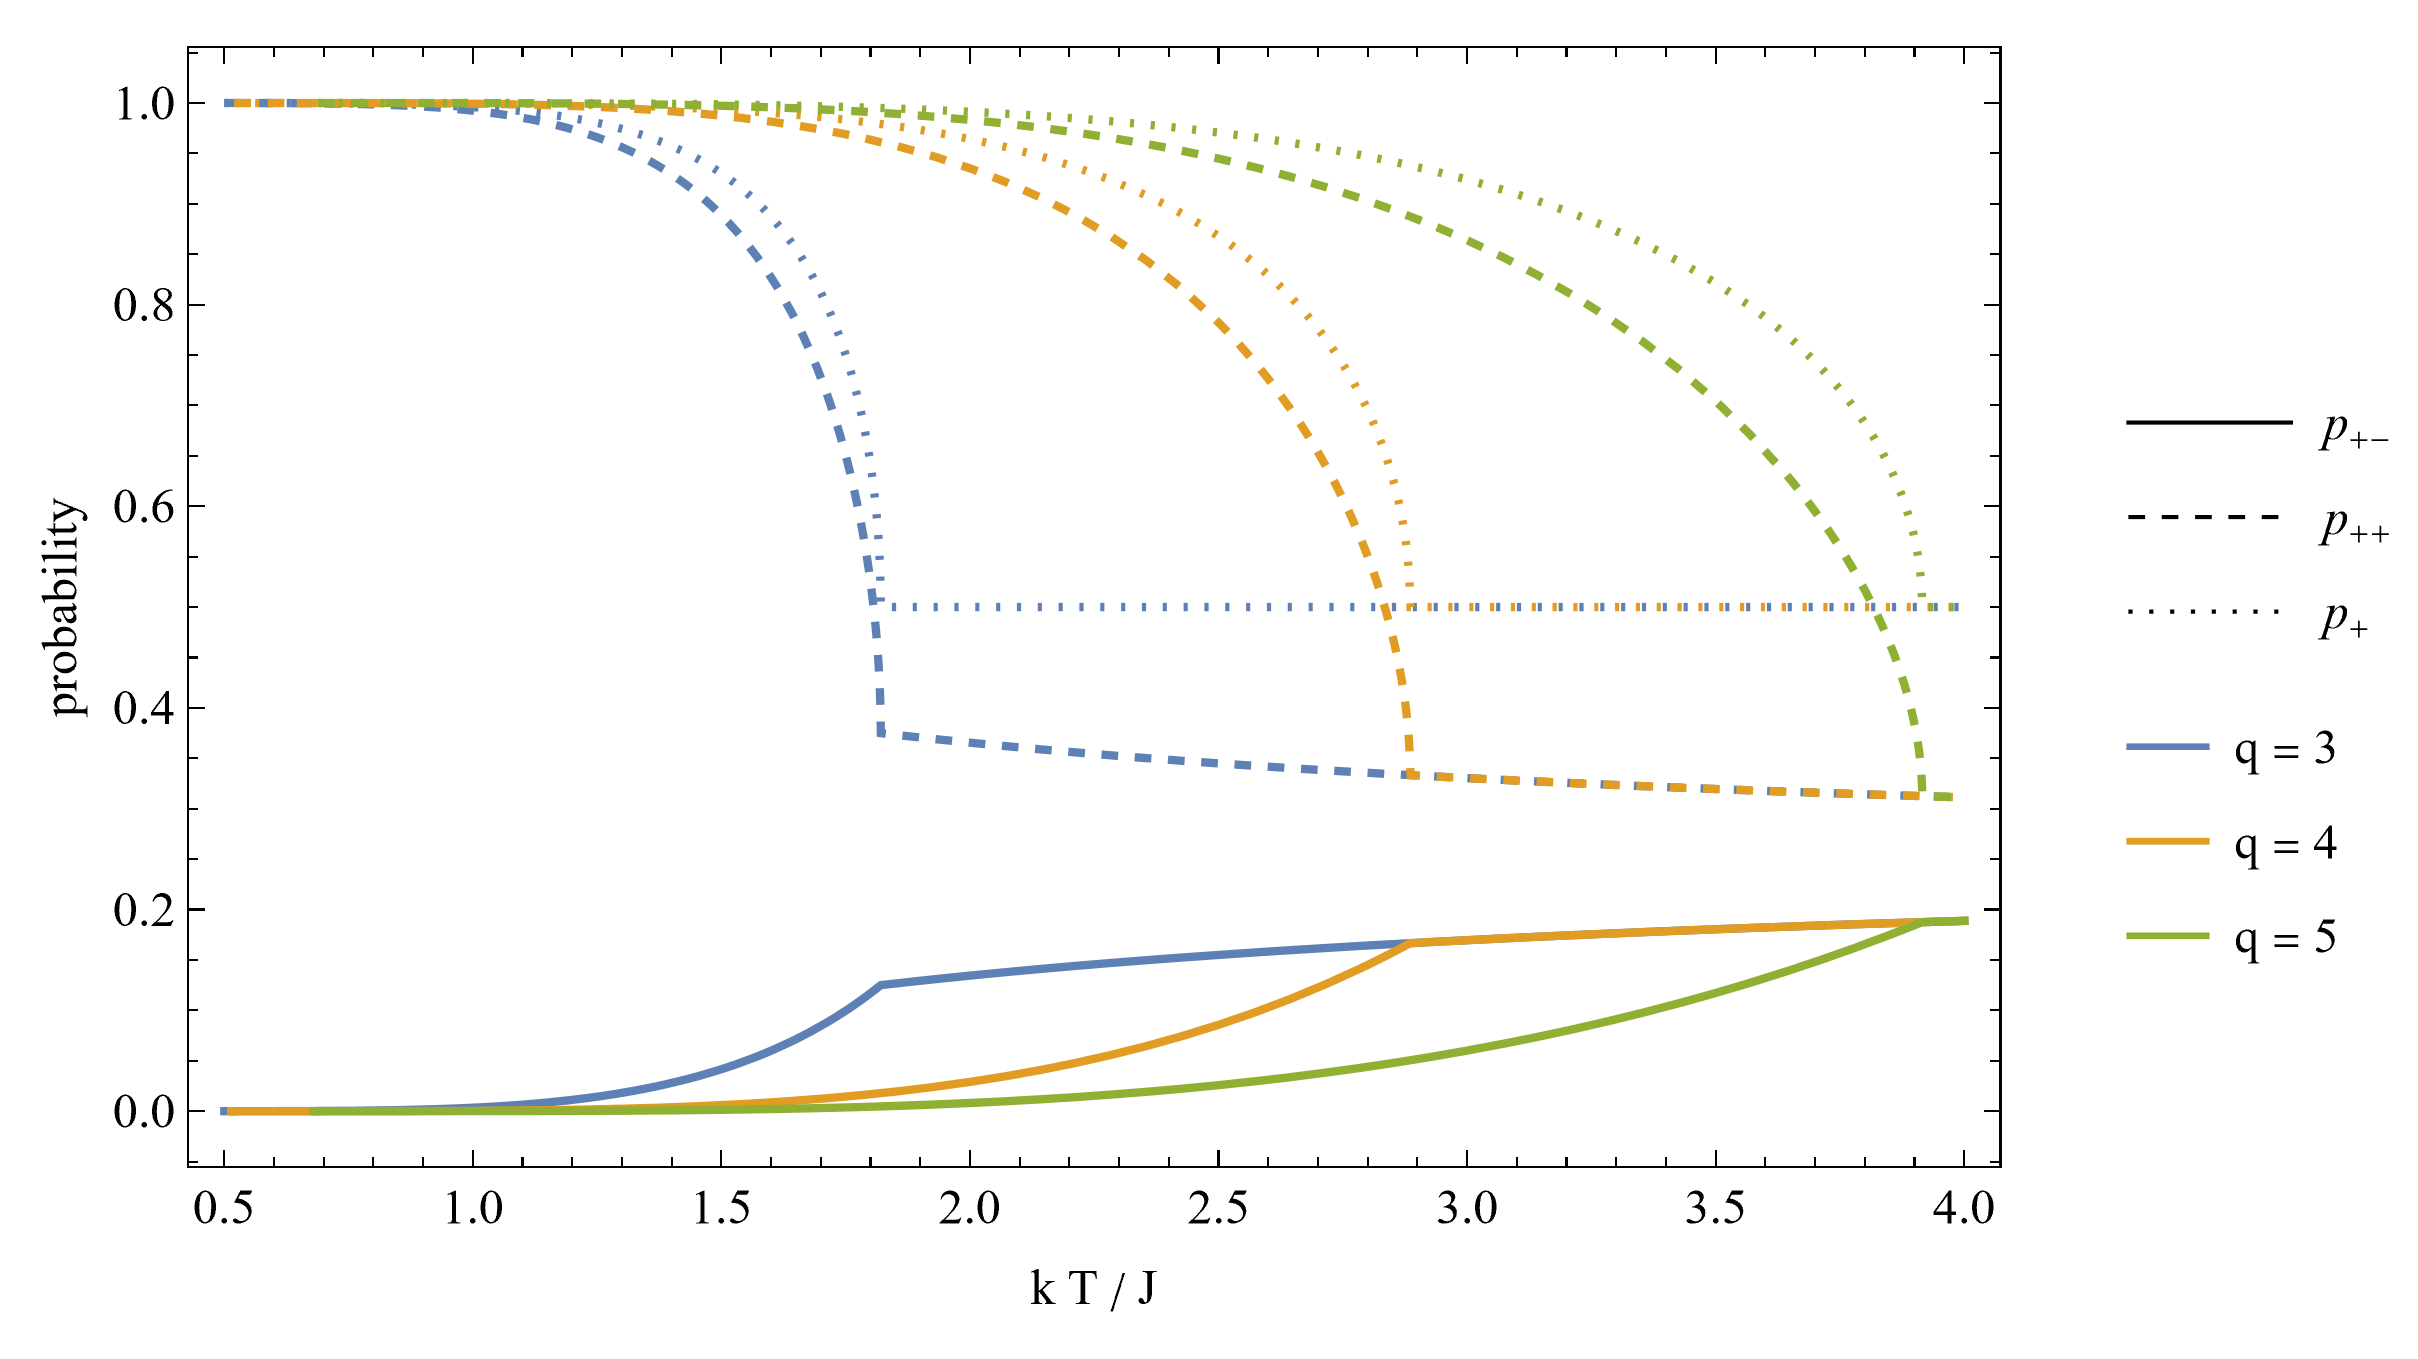
\includegraphics[width=\textwidth]{ising_model_fig/state_probability.png}
		\caption{状态概率}
		\label{各统计量随温度变化图-状态概率}
	\end{subfigure}
	\hfill
	\begin{subfigure}[b]{0.49\textwidth}
		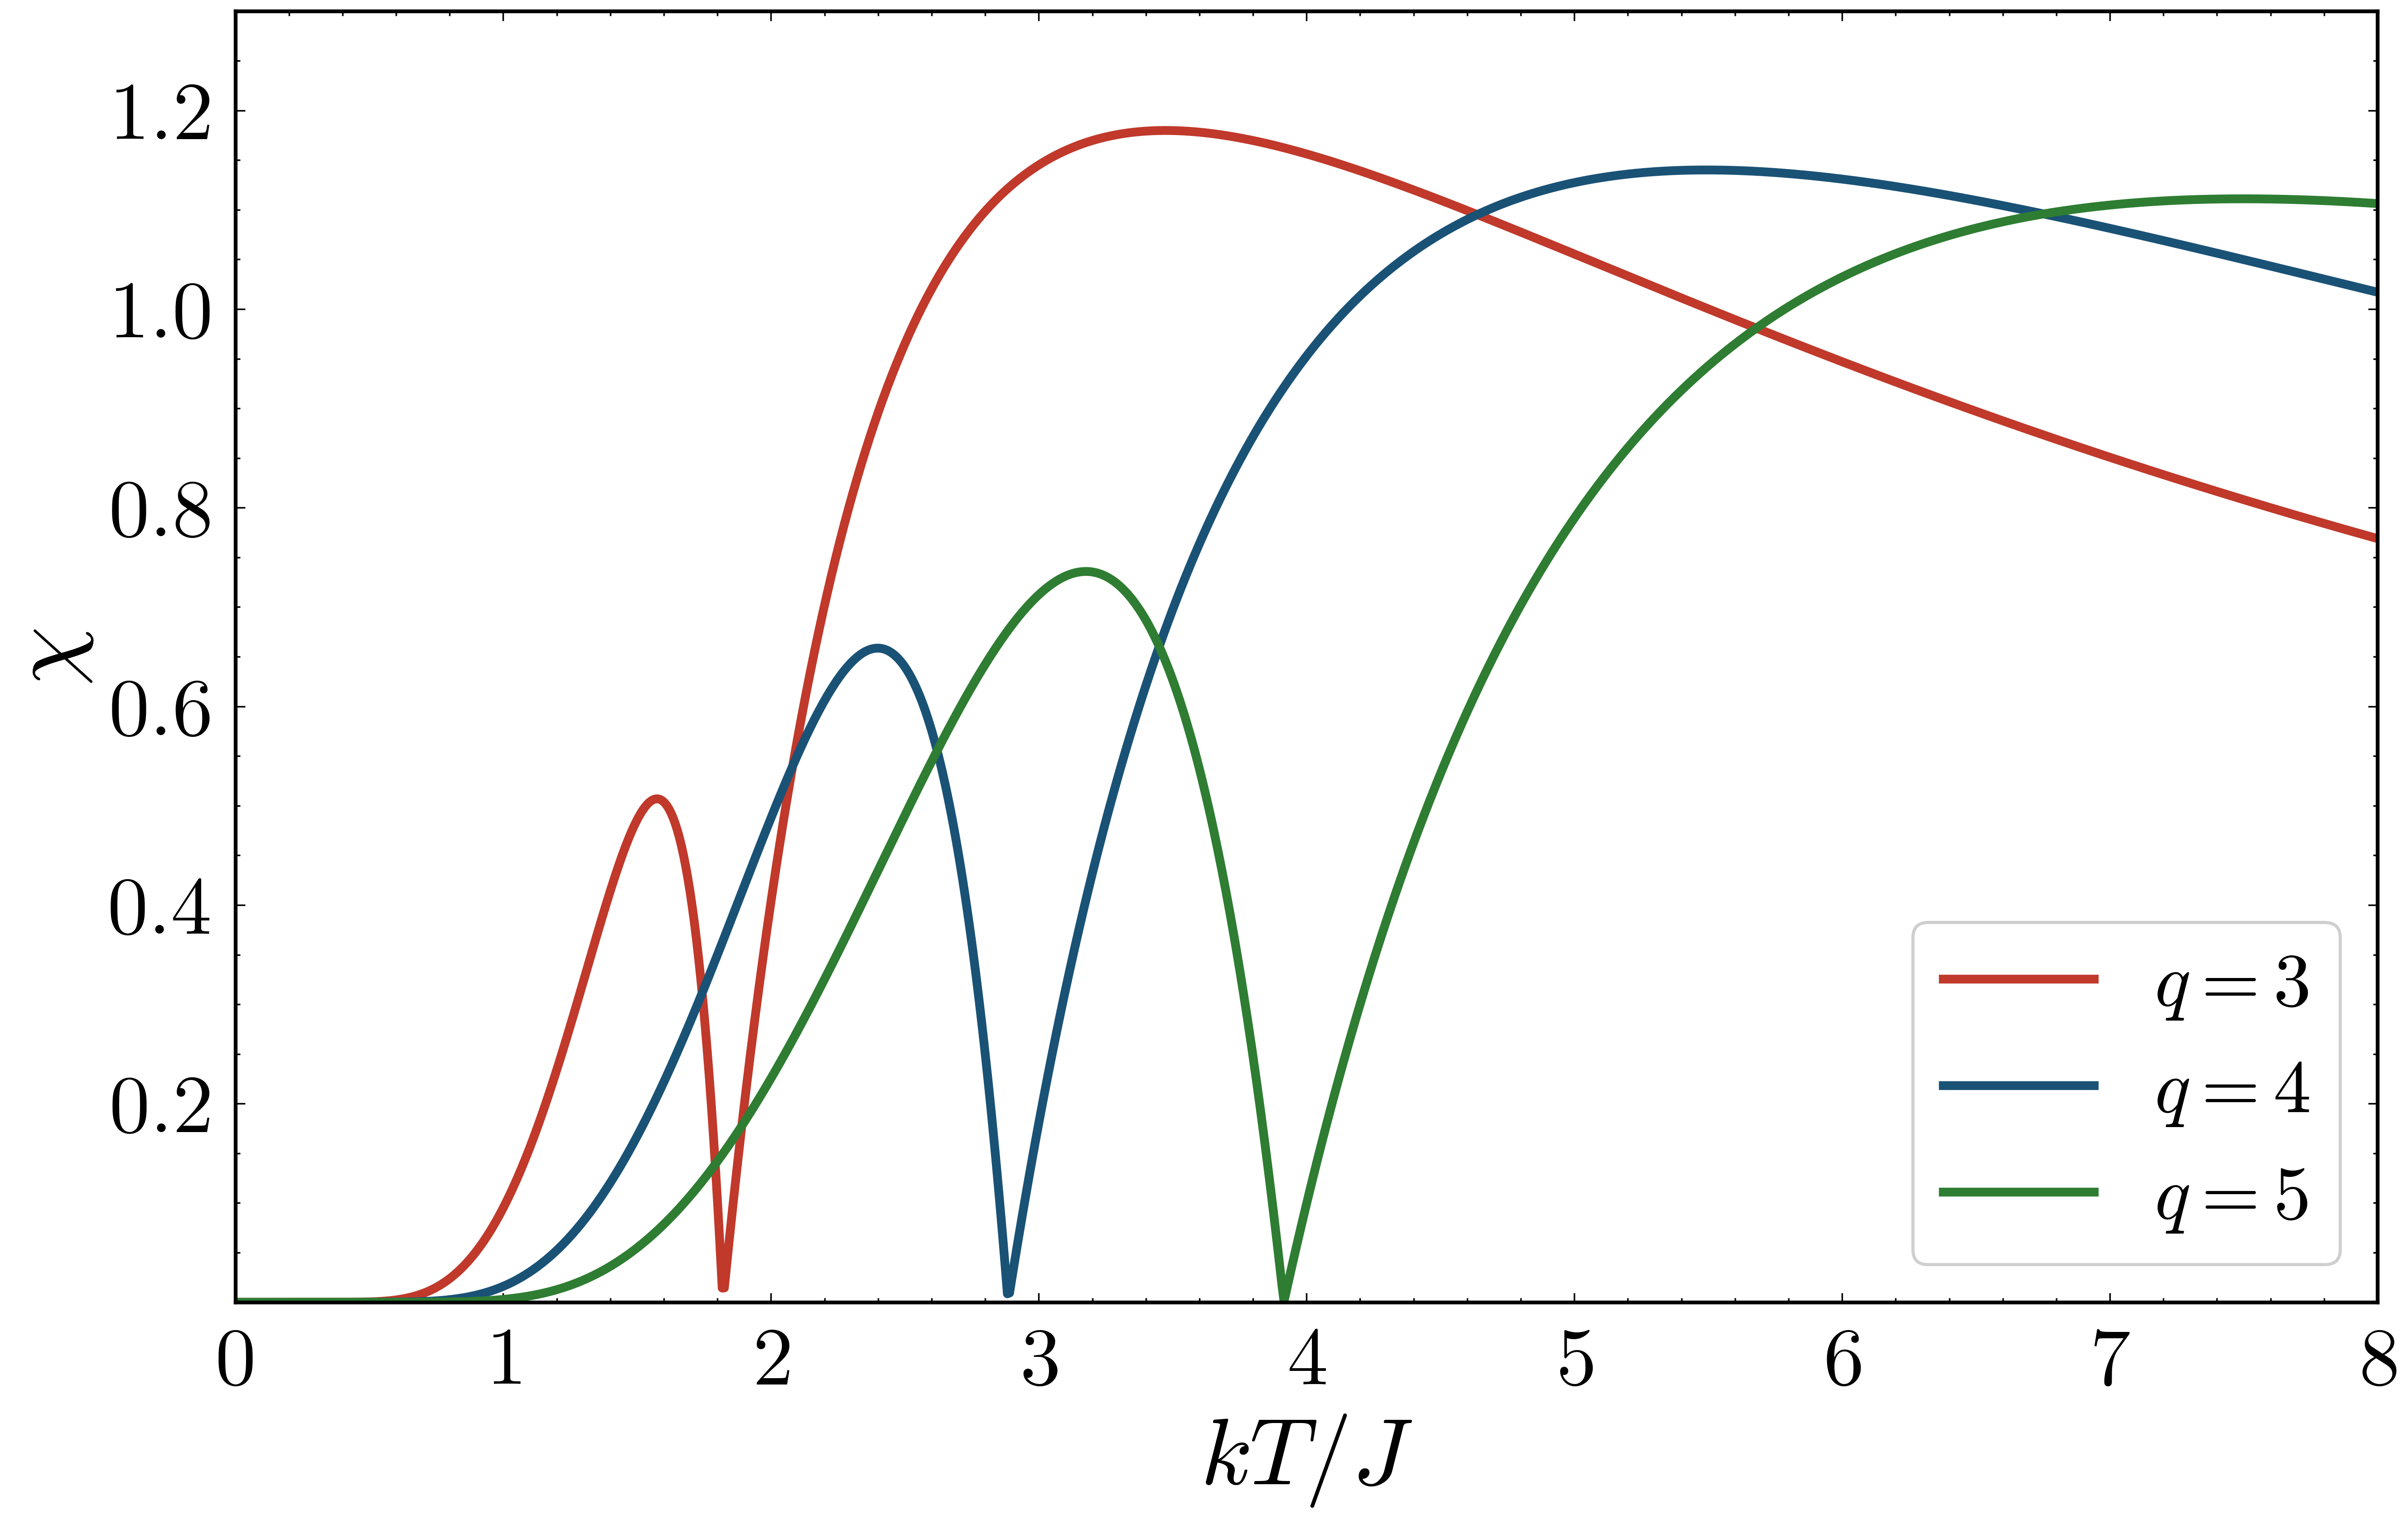
\includegraphics[width=\textwidth]{ising_model_fig/magnetic_susceptibility.png}
		\caption{磁化率}
		\label{各统计量随温度变化图-磁化率}
	\end{subfigure}

	\vspace{0.1cm}
	\begin{subfigure}[b]{0.49\textwidth}
		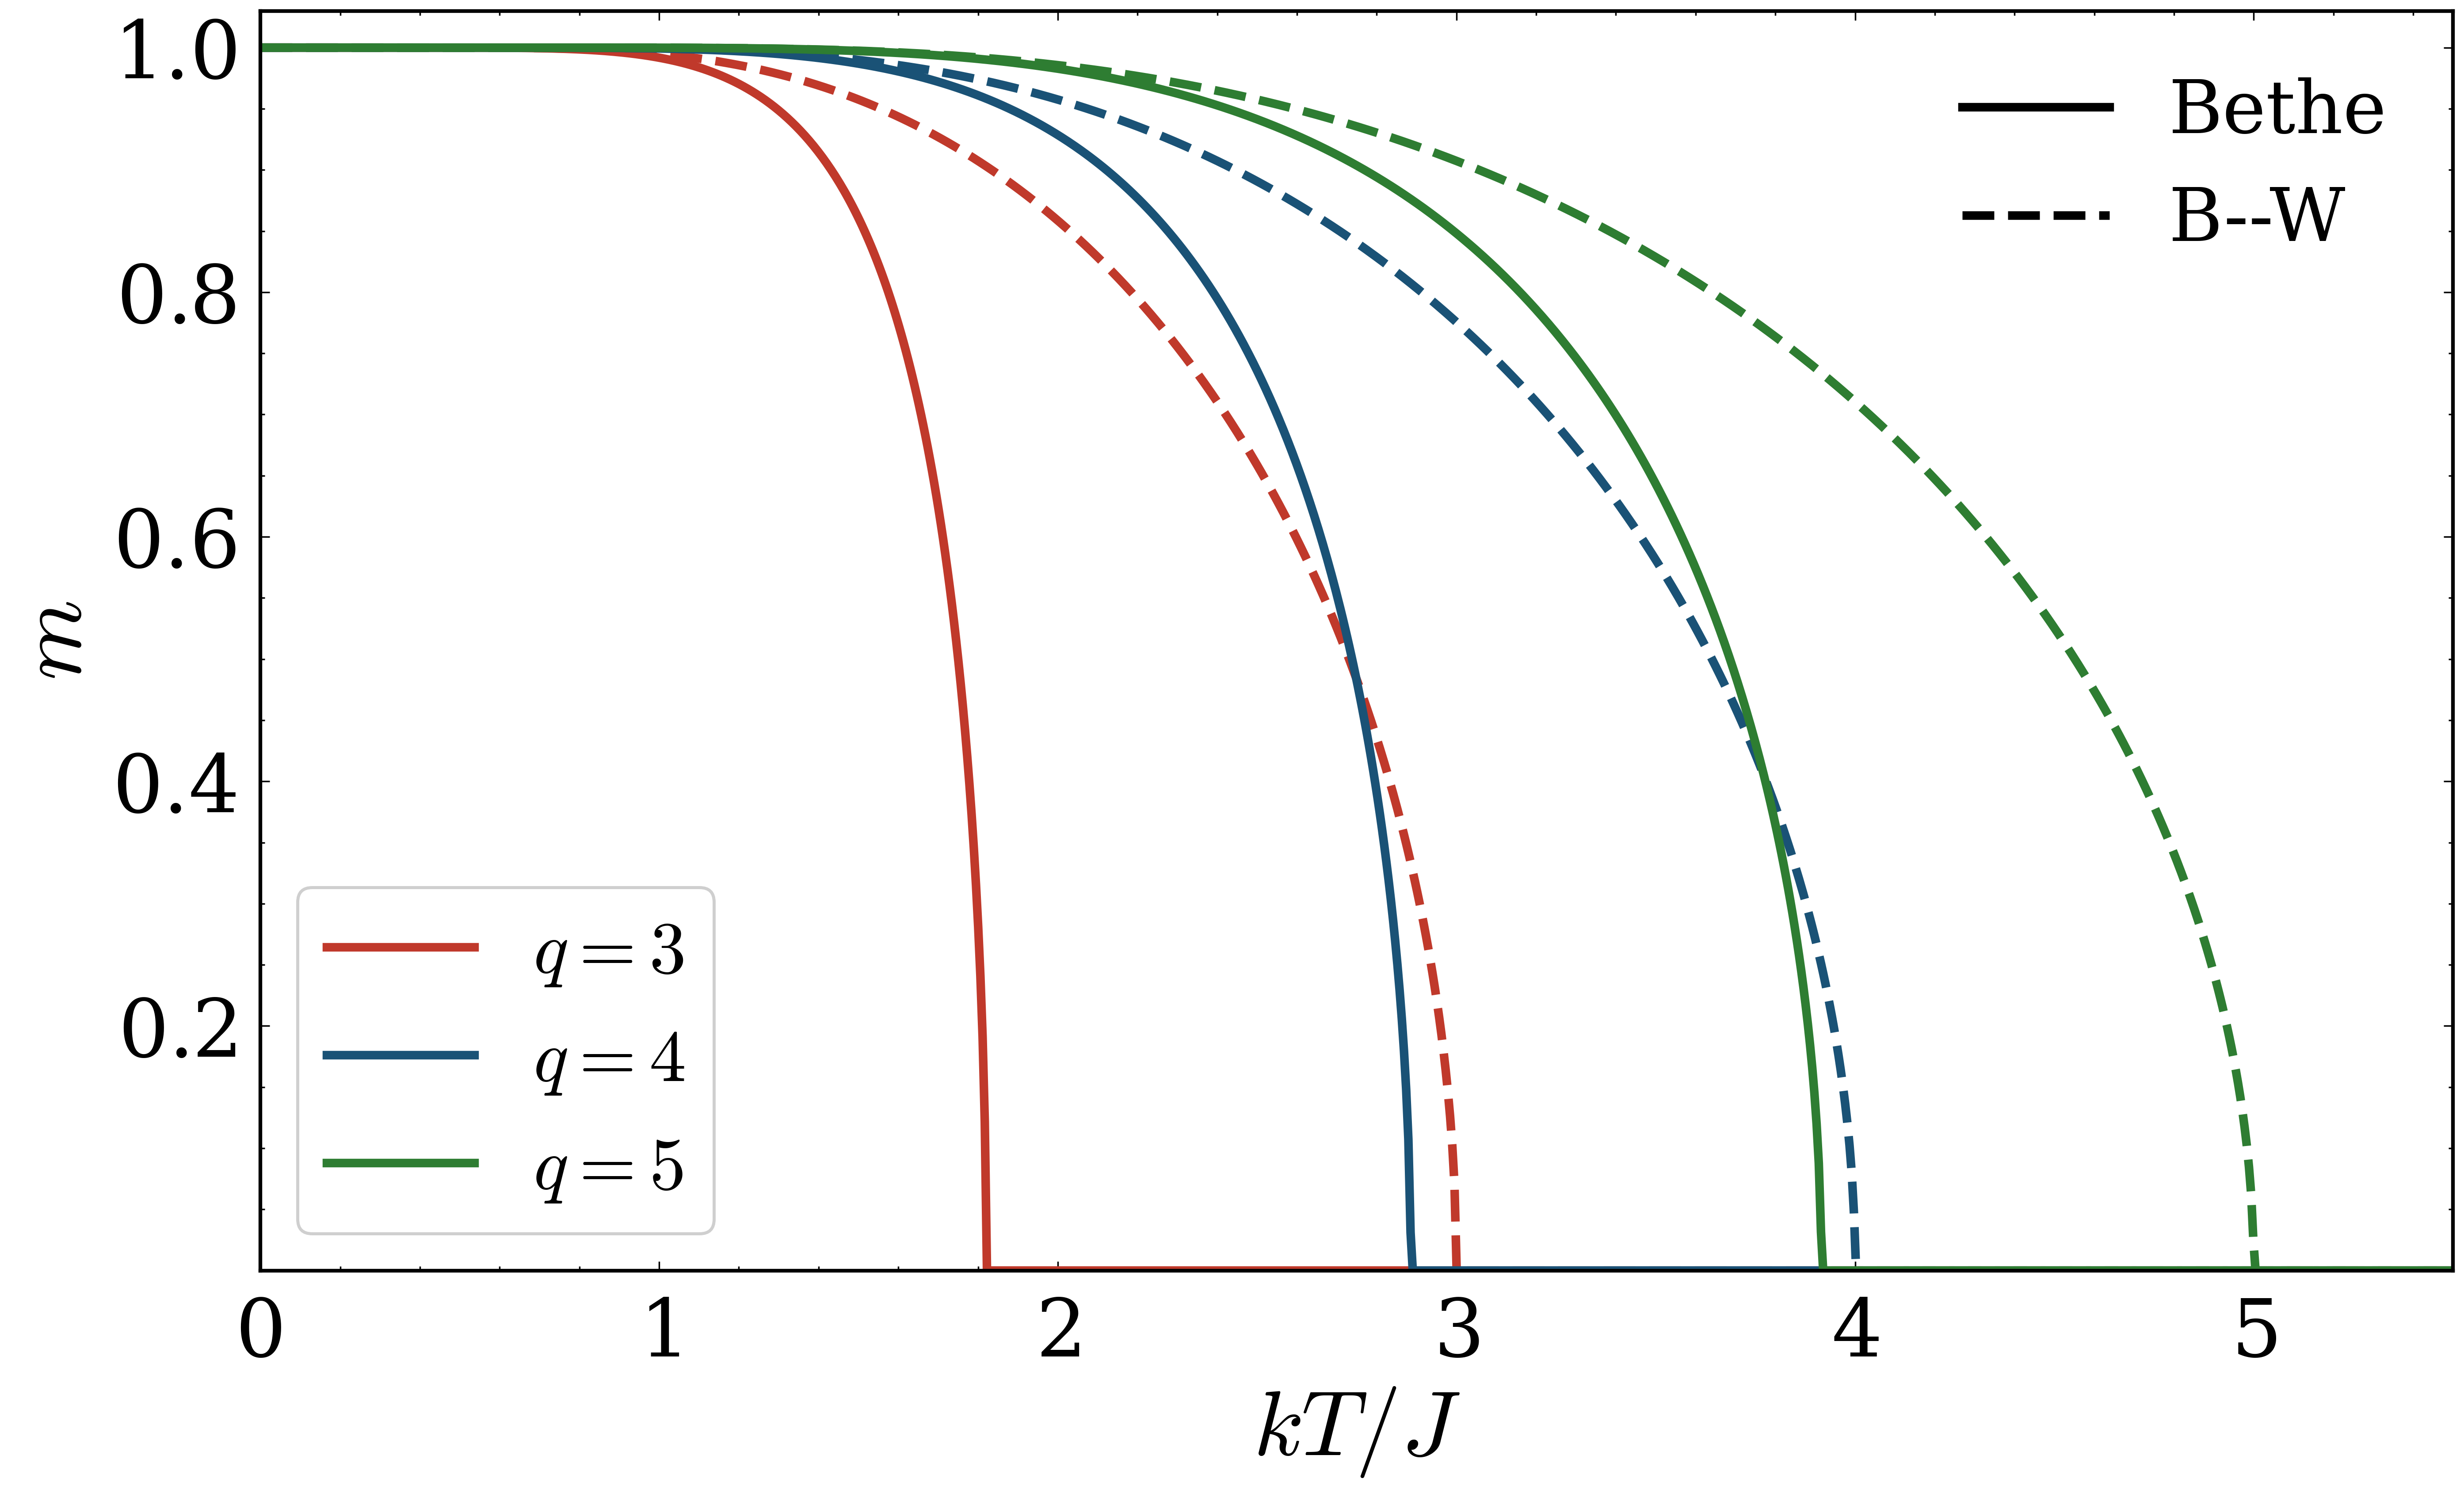
\includegraphics[width=\textwidth]{ising_model_fig/order_parameter.png}
		\caption{序参量}
		\label{各统计量随温度变化图-序参量}
	\end{subfigure}
	\hfill
	\begin{subfigure}[b]{0.49\textwidth}
		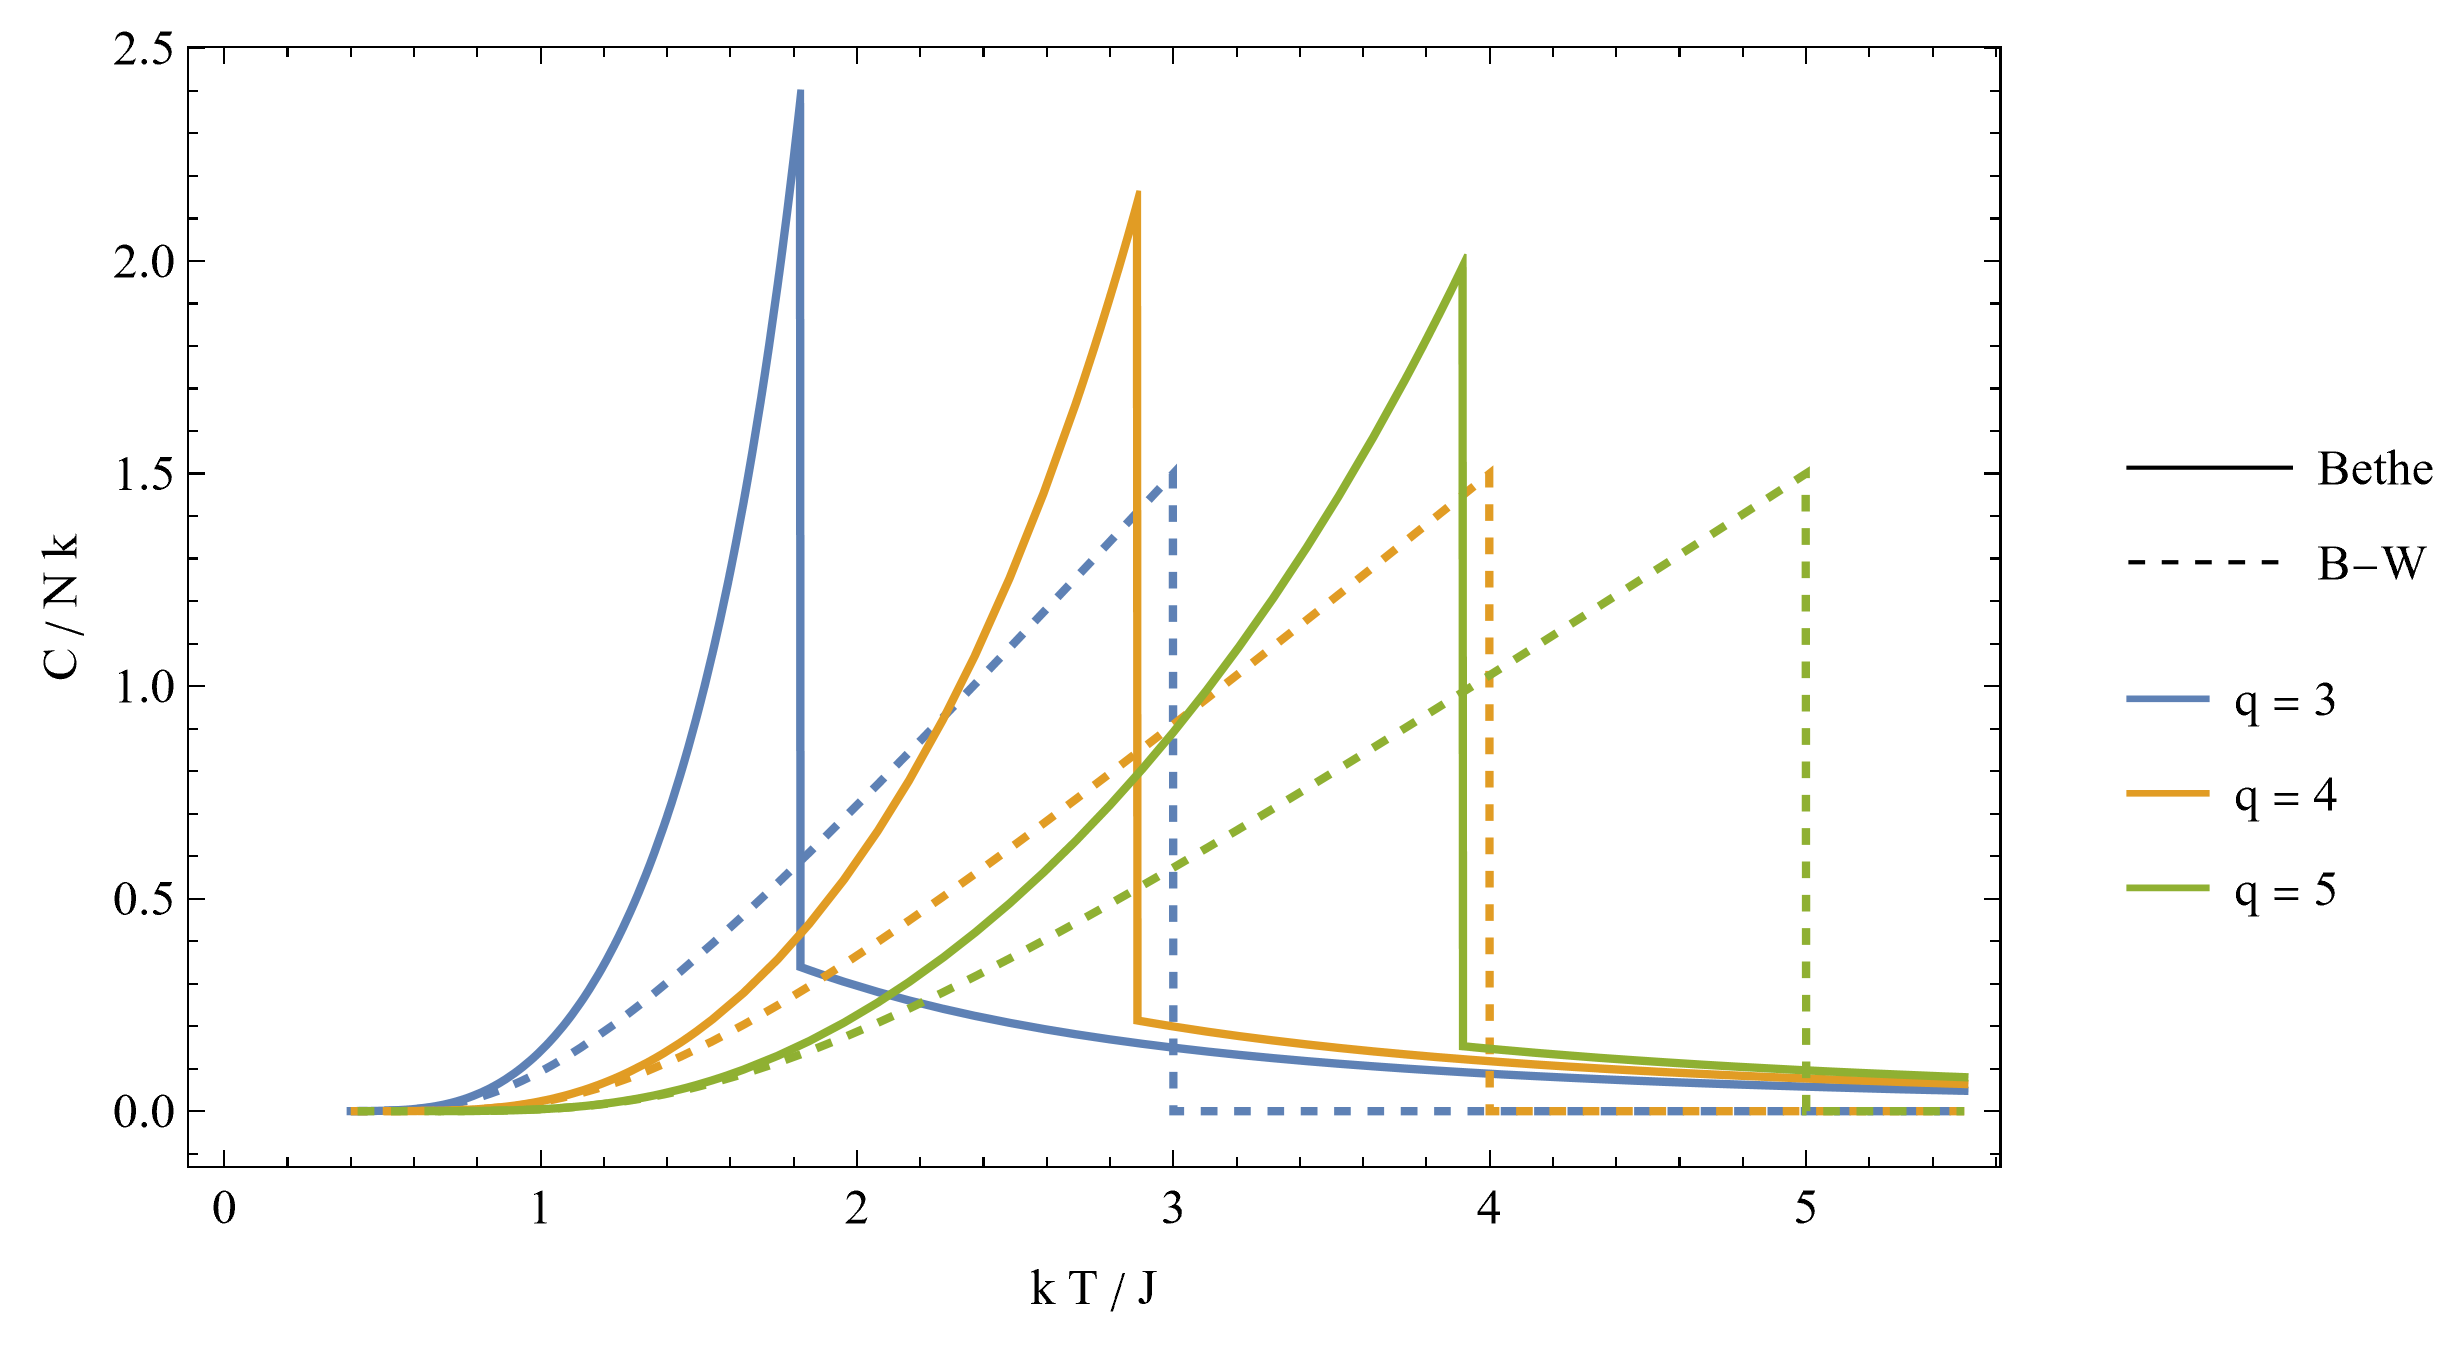
\includegraphics[width=\textwidth]{ising_model_fig/heat_capacity.png}
		\caption{热容}
		\label{各统计量随温度变化图-热容}
	\end{subfigure}
	\caption{Bethe 描述下各统计量随温度变化图}
	\label{各统计量随温度变化图}
\end{figure}

\subsection{一维链：树图方法的严格基准}

当 \(q=2\) 时，有限开边界链是树，Bethe 概率分解严格成立；周期边界链多出一条环，但在热力学极限中该单环的边界修正不影响自由能密度。此时不能直接使用 \(q>2\) 的 Bethe 临界温度公式，因为
\(\ln[q/(q-2)]\) 在 \(q=2\) 处发散，正确结论是不存在有限温度相变。

重新定义
\begin{equation*}
	\widetilde h=\frac{h}{1+t}=\frac{\mu B}{kT},\qquad
	\widetilde\chi=\chi(1+t),\qquad
\gamma=\frac J{kT}.
\end{equation*}
由上述自洽方程可得
\begin{align*}
a&=\frac12\,\mathrm{arcsinh}\left[
e^{2\gamma}\sinh\widetilde h
\left(\cosh\widetilde h+
\sqrt{e^{-4\gamma}+\sinh^2\widetilde h}\right)
\right],\\
m&=\frac{\sinh\widetilde h}
{\sqrt{e^{-4\gamma}+\sinh^2\widetilde h}},\\
\widetilde\chi
&=\frac{\cosh\widetilde h\,e^{-4\gamma}}
{\left(e^{-4\gamma}+\sinh^2\widetilde h\right)^{3/2}},\\
p_\pm&=\frac12\left[
1\pm\frac{\sinh\widetilde h}
{\sqrt{e^{-4\gamma}+\sinh^2\widetilde h}}\right].
\end{align*}
相邻成对概率为
\begin{align*}
p_{++}
&=\frac12\frac{e^{\widetilde h}
\left(\sqrt{e^{-4\gamma}+\sinh^2\widetilde h}
+\sinh\widetilde h\right)}
{\sqrt{e^{-4\gamma}+\sinh^2\widetilde h}
\left(\cosh\widetilde h+
\sqrt{e^{-4\gamma}+\sinh^2\widetilde h}\right)},\\
p_{--}
&=\frac12\frac{e^{-\widetilde h}
\left(\sqrt{e^{-4\gamma}+\sinh^2\widetilde h}
-\sinh\widetilde h\right)}
{\sqrt{e^{-4\gamma}+\sinh^2\widetilde h}
\left(\cosh\widetilde h+
\sqrt{e^{-4\gamma}+\sinh^2\widetilde h}\right)},\\
p_{+-}
&=\frac12\frac{e^{-4\gamma}}
{\sqrt{e^{-4\gamma}+\sinh^2\widetilde h}
\left(\cosh\widetilde h+
\sqrt{e^{-4\gamma}+\sinh^2\widetilde h}\right)}.
\end{align*}
并且
\begin{equation*}
\frac ENJ
=-\frac{
\sqrt{e^{-4\gamma}+\sinh^2\widetilde h}\cosh\widetilde h
+\sinh^2\widetilde h-e^{-4\gamma}}
{\sqrt{e^{-4\gamma}+\sinh^2\widetilde h}
\left(\cosh\widetilde h+
\sqrt{e^{-4\gamma}+\sinh^2\widetilde h}\right)}.
\end{equation*}
特别地，在 \(\widetilde h=0\) 时 \(m=0\) 对所有 \(T>0\) 成立，因此一维短程伊辛模型不存在有限温度自发磁化。这个例子也说明：树图上的局部严格性不自动意味着存在有限温度相变。

\subsection{Bragg--Williams 近似}

Bragg--Williams（B--W）近似把最近邻关联完全忽略，令
\begin{equation*}
	p_{\sigma\sigma'}=p_\sigma p_{\sigma'}.
\end{equation*}
于是
\begin{align*}
\frac EN
&=-\frac{qJ}{2}
\left(p_{++}+p_{--}-p_{+-}-p_{-+}\right)
-\mu B(p_+-p_-)\\
&=-\frac{qJ}{2}m^2-\mu Bm,\\
\frac S{Nk}
&=-\sum_\sigma p_\sigma\ln p_\sigma\\
&=-\frac{1+m}{2}\ln\frac{1+m}{2}
-\frac{1-m}{2}\ln\frac{1-m}{2}.
\end{align*}

对固定 \(q\) 的有限维晶格，B--W 直接舍弃最近邻关联。它在完全图的 \(N\to\infty\) 极限，或在 \(q\to\infty\) 且保持 \(qJ\) 有限的缩放极限下才成为受控描述。若采用完全图模型，耦合常数通常还需要随 \(N\) 缩放，以保证能量具有广延性。

在本小节重新以
\begin{equation*}
	T_c=T_c^{\mathrm{BW}}=\frac{qJ}{k},\qquad
	t=\frac{T-T_c}{T_c},\qquad
	h=\frac{\mu B}{kT_c}
\end{equation*}
定义无量纲变量，则
\begin{equation*}
\Phi=\frac F{NkT_c}
=-\frac12m^2-hm
+(1+t)\left[
\frac{1+m}{2}\ln\frac{1+m}{2}
+\frac{1-m}{2}\ln\frac{1-m}{2}
\right].
\end{equation*}
极值条件给出熟知的平均场自洽方程
\begin{equation*}
m=\tanh\left(\frac{m+h}{1+t}\right),
\qquad
\chi=\left(\frac{\partial m}{\partial h}\right)_t
=\frac{1-m^2}{t+m^2}.
\end{equation*}
在临界点附近
\begin{equation*}
h=tm+\mathcal O(m^3),\qquad
\left.m\right|_{t=0}=3^{1/3}h^{1/3}.
\end{equation*}
零场下
\begin{equation*}
\left[
m-\tanh\frac m{1+t}
\right]_{h=0}=0,
\qquad
\left.\frac E{NkT_c}\right|_{h=0}=-\frac12m^2,
\end{equation*}
\begin{equation*}
\left.\frac C{Nk}\right|_{h=0}
=\frac{m^2(1-m^2)}
{(1+t)(m^2+t)}.
\end{equation*}
临界点附近的两侧行为为
\begin{align*}
\left.m\right|_{h=0}
&=
\begin{cases}
0,&t\gtrsim0,\\
\pm\sqrt3(-t)^{1/2},&t\lesssim0,
\end{cases}
\qquad
\left.\chi\right|_{h=0}
=
\begin{cases}
t^{-1},&t\gtrsim0,\\
\frac12(-t)^{-1},&t\lesssim0,
\end{cases}\\
\left.\frac E{NkT_c}\right|_{h=0}
&=
\begin{cases}
0,&t\gtrsim0,\\
\frac32t,&t\lesssim0,
\end{cases}
\qquad
\left.\frac C{Nk}\right|_{h=0}
=
\begin{cases}
0,&t\gtrsim0,\\
\frac32,&t\lesssim0.
\end{cases}
\end{align*}
同样地，B--W 自由能的临界展开为
\begin{equation*}
\left.\Phi\right|_{t\to0,m\to0}
=-(1+t)\ln2-hm+\frac12tm^2+\frac1{12}m^4
+\mathcal O(t^3,t^2m^2,tm^4).
\end{equation*}
因此
\begin{equation*}
a_2=0,\qquad b_1=\frac12,\qquad c_0=\frac1{12},
\end{equation*}
并给出与 Bethe 解相同的临界指数，但不相同的临界温度、振幅和热容跃变。

从单点分布的角度，B--W 也可以写成
\begin{equation*}
	P_{\sigma_0}\propto
	\exp\left[\beta\sigma_0(\mu B+qJm)\right]
\quad\Longrightarrow\quad
m=\tanh\left(\frac{m+h}{1+t}\right),
\end{equation*}
其中 \(1+t=T/T_c=kT/(qJ)\)。这个写法把 B--W 的物理内容说得很清楚：所有邻居只通过平均磁化强度 \(m\) 产生一个均匀有效场，因此成对涨落被完全压平。
